In order to make predictions for the NEOCP in the era of LSST, we make simulated observations of a catalogue of solar system objects that takes into account currently known objects. We then use the \dig{} code to calculate NEO scores for each object and use these values to make predictions for the NEOCP. In the subsections below we explain each of these steps in more details.

\subsection{Hybrid Catalogue}
\subsection{Simulated Observations}
\subsection{\dig{} Score Calculation}
\subsection{LSST Discovery probability}
\todo{need to actually do this}

% \url{https://www.astroml.org/modules/generated/astroML.density_estimation.KNeighborsDensity.html#astroML.density_estimation.KNeighborsDensity}

% \url{https://docs.scipy.org/doc/scipy/reference/generated/scipy.spatial.cKDTree.query.html#scipy.spatial.cKDTree.query}

\begin{figure}
    \centering
    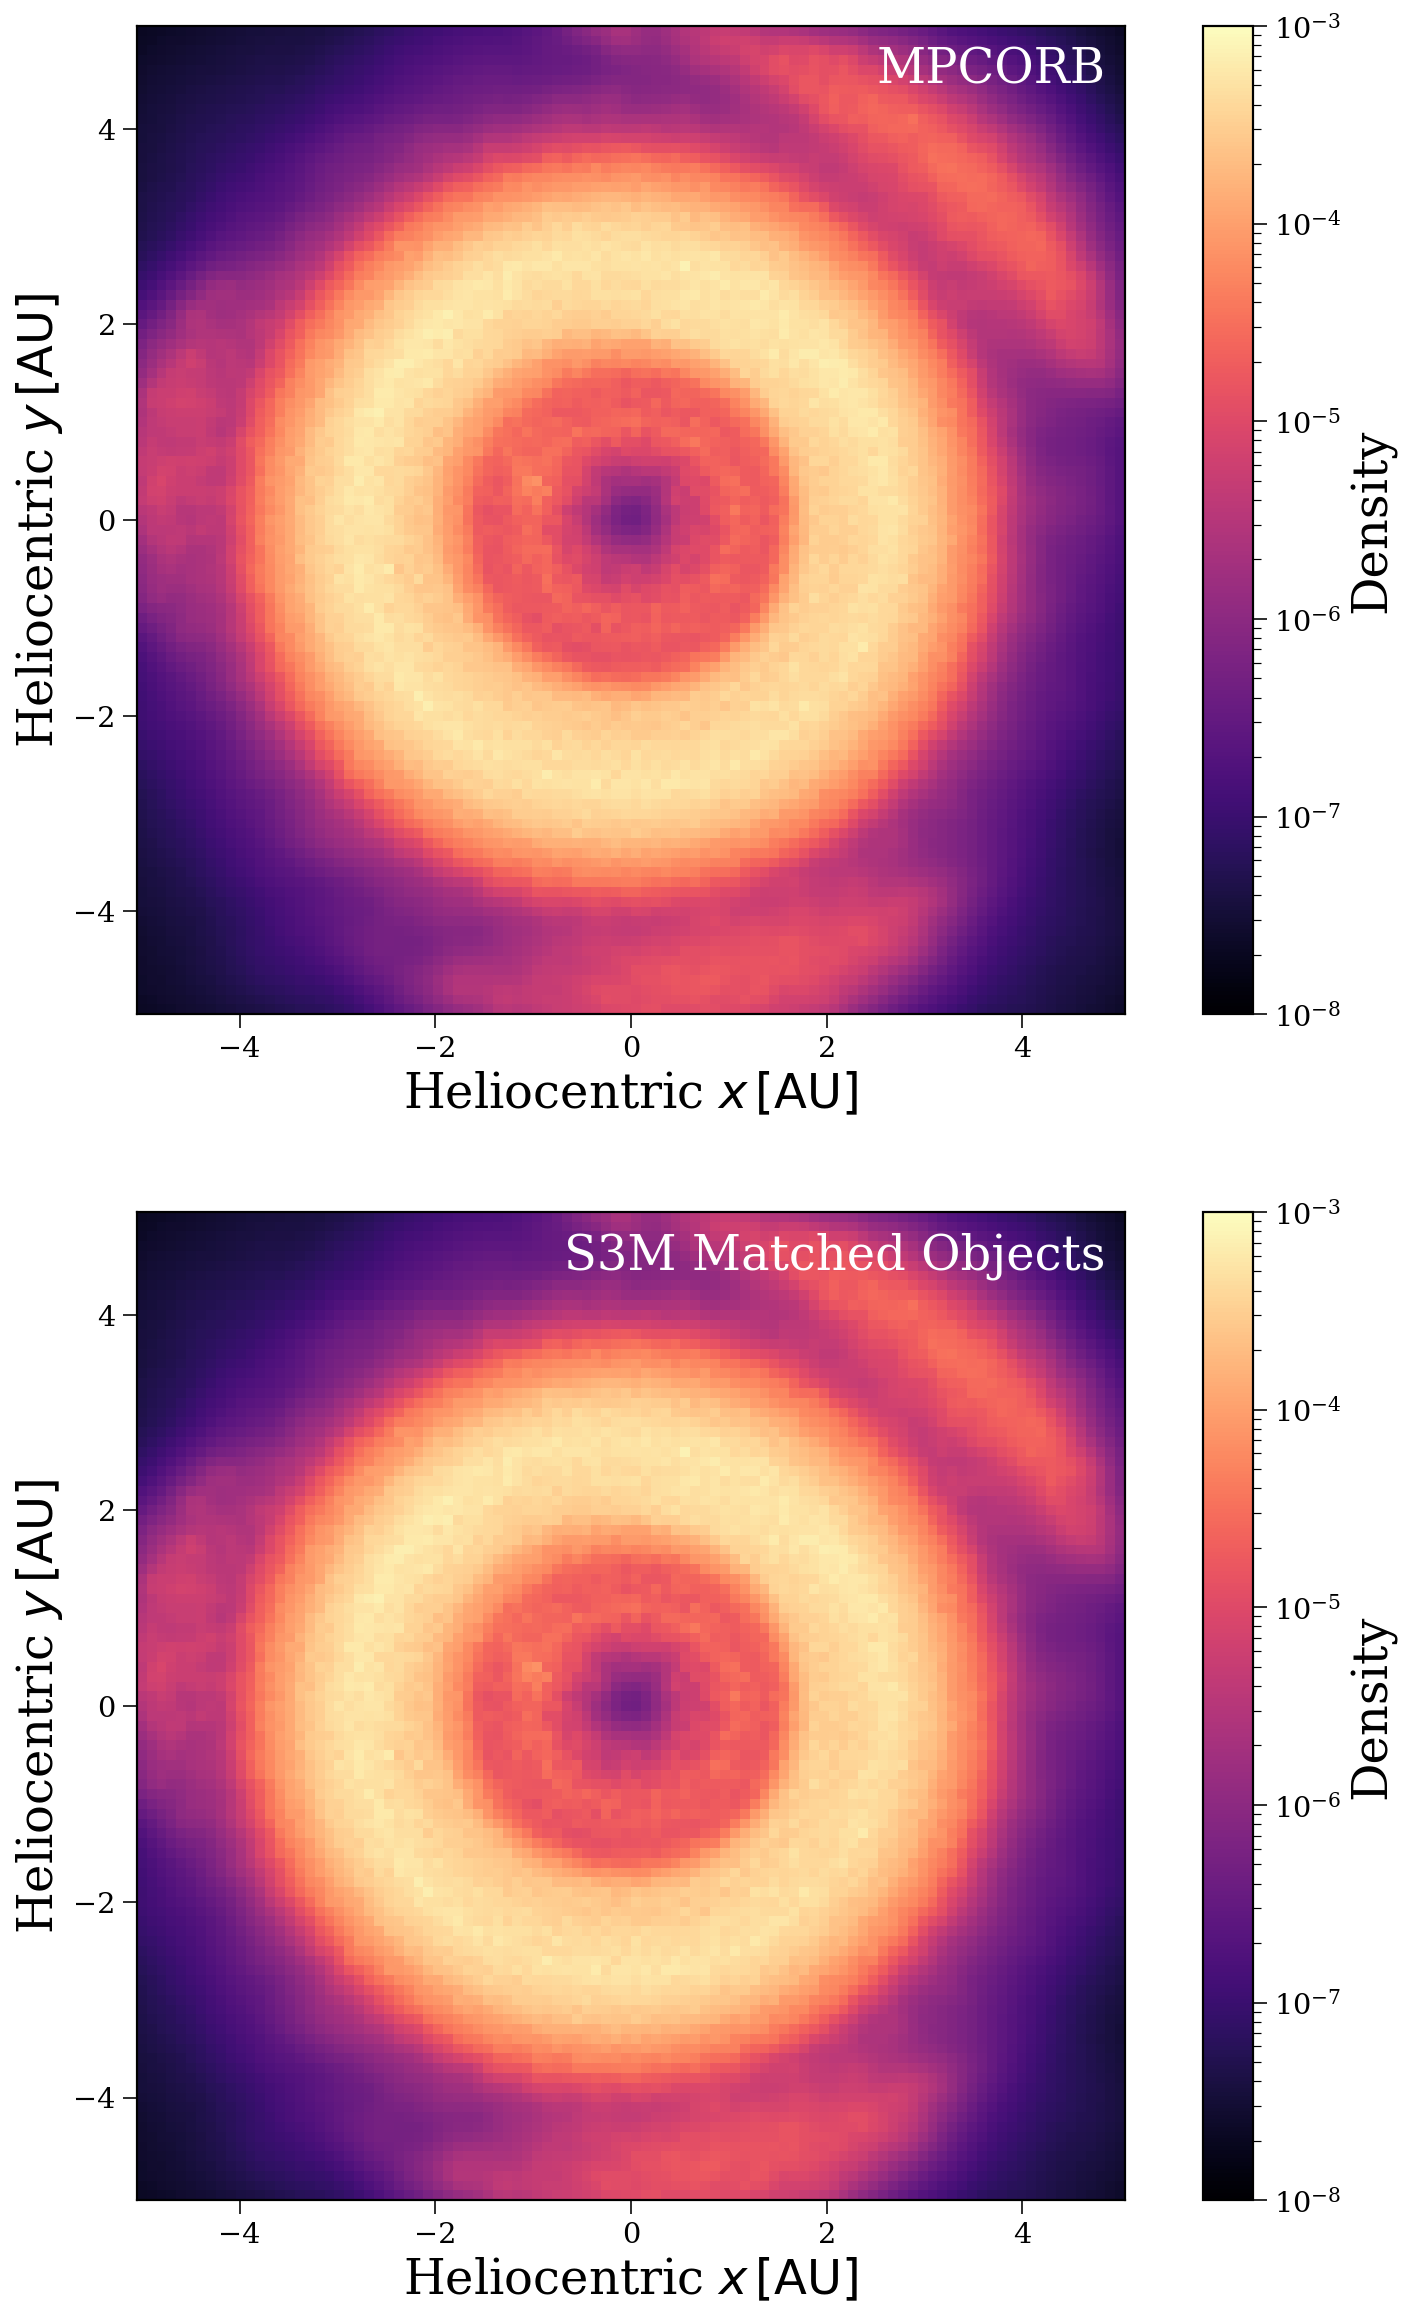
\includegraphics[width=\columnwidth]{density_comparisons.png}
    \caption{A comparison of the density of MPCORB objects with those objects that were matched by our hybrid catalogue algorithm.}
\end{figure}